% Modelo de monografia em LaTeX da UECE
%
% Na criação deste modelo foi tomada como base a dissertação de mestrado do
% Jeandro Bezerra, sem a ajuda dele este trabalho teria sido muito mais
% difícil. Este modelo utiliza o abnTeX e um pacote (uece.sty) para formatação
% de alguns anexos necessários da UECE (folha de rosto, CIP, epígrafe, ...).
%
% Este documento não clama possuir conformidade de 100\% com as normas de
% trabalhos da UECE. Consulte os guias oficiais.
%
% Autor do modelo: Rudy Matela
% Data do modelo: 20090920
% 
% Autor: Wesley Alcoforado
% Data: 22/02/2011

\documentclass[pnumabnt,normaltoc,espacoumemeio,capchap]{abnt}		
\usepackage[brazil]{babel}
\usepackage[utf8]{inputenc}
\usepackage{abnt-alf}
\usepackage{graphicx}
\usepackage{uece}
\usepackage{multicol}
\usepackage{lastpage}
\usepackage{enumerate}
\setcounter{secnumdepth}{3}
\setcounter{tocdepth}{3}
\usepackage[final]{pdfpages}

% Informações gerais do documento
\autor{Wesley Jefferson Oliveira Alcoforado}
\autorr{Alcoforado, Wesley Jefferson Oliveira}
\titulo{Mono-Manager - um gerenciador de trabalhos de conclusão de curso para o curso de Ciências de Computação da UECE}
\local{Fortaleza, Ceará}
\cidade{Fortaleza}
\data{2011}
\orientador{Mariela Cortés}
%\coorientador{Beltrano das Tantas e \par Cicrano da Silva}
\codigocip{A000z}{CDD:000.0}

% Descrição para folha de rosto
\comentario{
Monografia submetida à coordenação do curso de Ciências da Computação da Universidade Estadual do
Ceará, no ano de 2011, como requisito parcial para obtenção do grau de Bacharel em Ciências da Computação.
}

% Informações institucionais
\centro{Centro de Ciências e Tecnologia}
\curso{Graduação em Ciências da Computação}
\instituicao{Universidade Estadual do Ceará}

% Epígrafe: citação e autor
\epigrafe{``L'ordinateur obéit à vos ordres, pas à vos intentions.''}
\autorepigrafe{Anônimo}

% Membros da comissão avaliadora
\bancaum{Profª. Drª. \ABNTorientadordata\\Universidade Estadual do Ceará - UECE\\Orientador}
\bancadois{Prof. Dr. Beltrano das Tantas\\Universidade Estadual do Ceará - UECE\\Co-orientador}
\bancatres{Prof. Me. Cricrano da Silva\\Universidade Estadual do Ceará - UECE\\Co-orientador}
\bancaquatro{Prof. Dr. Zé Ninguém\\Universidade Estadual do Ceará - UECE}

% Palavras chave
\pcs{TCC}{Processo}{Informatização}
\kws{TCC}{Processo}{Informatização}

\begin{document}

\capa
\folhaderosto
\makecippage
\termodeaprovacao

\pretextualchapter{Agradecimentos}
À minha esposa Raquel por ter me incentivado a escrever minha monografia, me apoiando nos
momentos em que fraquejei.

Aos amigos de graduação mais próximos pelo apoio mútuo durante toda a jornada na universidade.

Aos professores por terem compartilhado seus conhecimentos conosco.
\pagebreak

\makeepigrafe
\tableofcontents
\listadefiguras
\listadetabelas
% \listadesiglas % \sigla{sigla}{Descrição}
% \listadesimbolos % \simbolo{símbolo}{Descrição}

\begin{resumo}
\noindent
Este trabalho tem como objetivo apresentar uma ferramenta que informatiza
o processo de avaliação de trabalhos de conclusão da graduação em Ciências 
da Computação da Universidade Estadual do Ceará. Essa ferramenta foi projetada 
para minimizar a quantidade de documentos impressos e para proporcionar uma 
visão geral do andamento das atividades. Além disso, ela é capaz de notificar 
as pessoas envolvidas automaticamente, alertando sobre o cumprimento dos prazos.
\noindent
\palavraschave
\end{resumo}
\pagebreak

\chapter{Introdução}
Através da informatização de processos, é possível otimizar tarefas que demandam tempo, 
um bem escasso, e também diminuir a quantidade de documentos impressos nas nossas mesas, 
papéis que muitas vezes se perdem no meio de outros documentos.

\section{Motivação}
No último semestre do curso de Ciências da Computação existe a disciplina de Projeto Final, 
a qual é regida por um regulamento e possui todo um processo burocrático que pode ser informatizado, 
de forma a organizar melhor as tarefas dos professores e alunos envolvidos.

A construção de um sistema que gerencie o processo de submissão de projetos ajudaria 
não apenas na organização dos documentos e datas, mas também possibilitaria aos 
orientadores e à Comissão de Projeto Final ter um controle dos alunos que, por um 
motivo ou outro, não sabem por onde começar ou estão parados no meio do caminho, 
além de manter todos informados sobre o andamento dos seus projetos.

\section{Objetivo}
Com a construção de um sistema de gerenciamento de submissão de projetos, 
espera-se uma diminuição no esforço despendido na organização e um maior 
controle sobre os documentos, datas, alunos e professores envolvidos.

\section{Metodologia}

Para o desenvolvimento deste trabalho foram inicialmente construídos casos de usos 
simplificados, onde as funcionalidades foram expostas com mais clareza, mas sem 
muito aprofundamento para garantir que o projeto fosse concluído em tempo hábil. 

A partir dos casos de uso, o banco de dados foi modelado, assim como as classes 
de acesso a dados.

Após o término da modelagem, foi iniciada a fase de codificação dos casos de uso, 
seguidos pelo desenvolvimento do design da aplicação.

Por último foram realizados testes de aceitação e correções de bugs encontrados.

Para a construção dessa aplicação foi utilizada a linguagem de script \sigla{PHP}{PHP: Hypertext Preprocessor}, na 
sua versão 5.3.3 em conjunto com o framework Symfony 1.4.2. Como IDE, foi utilizado 
o NetBeans 6.9, um framework para desenvolvimento e testes com PHP. O 
banco de dados escolhido foi o PostgreSQL versão 8.4.

Estas ferramentas foram escolhidas devido a serem gratuitas e possuirem versões 
estáveis para Linux, que é a plataforma onde se pretende implantar a versão 
final da aplicação. Mais detalhes sobre as tecnologias são expostas na seção ~\ref{tecnologias}.

\section{Organização do trabalho}

Além deste capítulo introdutório, o presente trabalho consiste em mais 4 capítulos. 
No capítulo ~\ref{cha:regulamento} é feita uma apresentação do processo de 
entrega de \sigla{TCC}{Trabalho de Conclusão de Curso}s na UECE, de acordo
com o regulamento da instituição. No capítulo ~\ref{cha:desenvolvimento} é descrito como foi o processo de desenvolvimento 
da aplicação, assim como a organização do banco de dados e os requisitos do sistema. 
O capítulo ~\ref{cha:utilizacao} demonstra como utilizar o sistema. O capítulo ~\ref{cha:conclusoes} apresenta as conclusões
e uma breve discussão sobre trabalhos futuros.


\chapter{Regulamento de Projeto Final}

O processo de submissão e avaliação de projetos finais no curso
de Ciências da Computação da UECE segue um regulamento que normatiza 
o tipo do conteúdo da monografia, o procedimento para o desenvolvimento 
e para a aprovação do projeto, a constituição da Comissão de Projeto 
Final e as atribuições desta, do orientador e do aluno. 

\section{Entidades envolvidas e suas atribuições}
O desenvolvimento do projeto final deve ser desempenhado individualmente
pelo aluno, sob a orientação de um docente, o orientador. O orientador deve
ser um docente lotado no curso de Ciências da Computação da UECE, seja ele
professor efetivo, substituto ou visitante. O aluno pode ainda contar com a
colaboração de co-orientadores, podendo estes serem docentes da UECE ou de 
outras IES (Instituição de Ensino Superior) ou ainda profissionais com graduação
plena em Ciências da Computação ou cursos afins e com no mínimo 3 (três) anos
de experiência em orientação de alunos ou coordenação de projetos.

A Comissão de Projeto Final, ou simplesmente Comissão,  é o órgão 
responsável pelo acompanhamento do processo de desenvolvimento do projeto final. 
Ela é composta por 3 (três) docentes efetivos pertencentes ao curso de 
Bacharelado em Ciência da Computação da UECE, havendo ainda 2 (dois) membros 
suplentes, sendo todos esses (permanentes e suplentes) escolhidos através de 
eleição no Colegiado do curso de Ciência da Computação e nomeados pelo 
Coordenador da graduação. O membro da Comissão fica impedido de emitir 
parecer sobre o trabalho de seus orientandos, que, neste caso, 
deverão ser avaliados por um membro suplente.

Compete ao aluno:
\begin{enumerate}[a.]
\item elaborar projeto de Proposta de Projeto Final;
\item conduzir e executar o Projeto Final;
\item cumprir os prazos estabelecidos no cronograma pré-estabelecido;
\item redigir e defender o Projeto Final;
\item entregar cópia corrigida do Projeto Final à secretaria;
\item tomar ciência dos prazos estabelecidos pela Comissão de Projeto Final e cumpri-los.
\end{enumerate}

Compete ao orientador e co-orientador:
\begin{enumerate}[a.]
\item orientar o aluno na organização de seu plano de estudo, pesquisa e assistí-lo na preparação da monografia;
\item viabilizar a realização do Projeto Final;
\item encaminhar a Proposta de Projeto Final e a Solicitação de Defesa à Comissão;
\item propor à Comissão a composição da Banca Examinadora;
\item encaminhar a Ata de Defesa, devidamente preenchida e assinada, ao Coordenador do curso.
\end{enumerate}

Compete à Comissão:
\begin{enumerate}[a.]
\item aprovar a proposta e plano de trabalho de Projeto Final;
\item aprovar as indicações dos orientadores de Projeto Final que não sejam docentes do curso;
\item aprovar os membros das bancas avaliadoras do Projeto Final;
\item autorizar a defesa de monografia de Projeto Final;
\end{enumerate}

\subsection{Blih blih blih} 
 
Asdf qwer zxcv asdf qwer zxcv.
Asdf qwer zxcv asdf qwer zxcv.
Asdf qwer zxcv asdf qwer zxcv.
Asdf qwer zxcv asdf qwer zxcv.
Asdf qwer zxcv asdf qwer zxcv.
Asdf qwer zxcv asdf qwer zxcv.
Asdf qwer zxcv asdf qwer zxcv.


\section{Test 1 2 3 4}
\label{sec:lateracao}
 
Asdf qwer zxcv asdf qwer zxcv.
Asdf qwer zxcv asdf qwer zxcv.
Asdf qwer zxcv asdf qwer zxcv.
Asdf qwer zxcv asdf qwer zxcv.
Asdf qwer zxcv asdf qwer zxcv.


\subsection{Figura}

A figura \ref{fig:graph} mostra uma figura. Quidquid latine dictum sit altum
viditur. The quick brown fox jumps over the lazy dog. Quidquid latine dictum
sit altum viditur. The quick brown fox jumps over the lazy dog.

\begin{figure}[htbp]
\centering

\includegraphics[width=.30\textwidth]{fig/uece}
\caption{Brasão da UECE}
\label{fig:graph}
\end{figure}


\subsection{Tabela}

A tabela \ref{tab:tabela} mostra uma tabela. Quidquid latine dictum sit altum
viditur. The quick brown fox jumps over the lazy dog. Quidquid latine dictum
sit altum viditur. The quick brown fox jumps over the lazy dog.

\begin{table}[htbp]
	\caption{Tabela}
	\label{tab:tabela}
	\centering
	\begin{tabular}{|c|l|r|}
		\hline
		The 	&	Quick 	&	Brown	\\
		\hline
		Fox	&	Jumps	&	Over	\\
		The	&	Lazy	&	Dog	\\
		\hline 
	\end{tabular}
\end{table} 


\subsection{Citações (Referências)}

De acordo com \cite{DEAD:1666,BEEF:1234} este paragrafo exemplifica referências
(citações). Lorem ipsum dolor sit amet, consectetur adipisicing elit, sed do
eiusmod tempor incididunt ut labore et dolore magna aliqua. Ut enim ad minim
veniam, quis nostrud exercitation ullamco laboris nisi ut aliquip ex ea commodo
consequat. Duis aute irure dolor in reprehenderit in voluptate velit esse
cillum dolore eu fugiat nulla pariatur. Excepteur sint occaecat cupidatat non
proident, sunt in culpa qui officia deserunt mollit anim id est laborum.
Quidquid latine dictum sit altum viditur.


\bibliographystyle{abnt-alf}
\bibliography{bib}
\appendix
\chapter{Apêndice}
\clearpage
\section{Casos de uso}
\subsection{Manter Professores}
\begin{longtable}{r p{12cm}}
\hline
Atores & Administrador \\ \hline
Pré-condições & O administrador deve estar logado no sistema.\\ \hline
Fluxo básico &1. O caso de uso se inicia quando o administrador seleciona manter professores no menu do sistema. \newline
                2. Uma vez que o administrador seleciona uma das opções disponíveis (incluir, alterar, excluir, listar): \newline
                \hspace*{1cm} a) Se o administrador selecionar a opção incluir, o caso de uso segue para o sub-fluxo 2 - Incluir Professor. \newline 
                \hspace*{1cm} b) Se o administrador selecionar a opção alterar, o caso de uso segue para o sub-fluxo 3 - Alterar Professor.  \newline 
                \hspace*{1cm} c) Se o administrador selecionar a opção excluir, o caso de uso segue para o sub-fluxo 4 - Excluir Professor.  \newline 
                \hspace*{1cm} d) Se o administrador selecionar a opção listar, o caso de uso segue para o sub-fluxo 5 - Listar Professores.  \newline 
                3. O caso de uso se encerra. \newline \\
Incluir Professor & 1. Este sub-fluxo se inicia quando o administrador seleciona incluir um novo professor. \newline
                    2. O sistema exibe os seguintes campos (os campos com asterisco são obrigatórios): \newline
                    \hspace*{1cm} * Nome de usuário \newline
                    \hspace*{1cm} * Email \newline
                    \hspace*{1cm} * Senha \newline
                    \hspace*{1cm} * Confirmação de senha \newline
                    \hspace*{1cm} Nome \newline
                    \hspace*{1cm} Sobrenome \newline
                    \hspace*{1cm} * Instituição \newline
                    \hspace*{1cm} * Titulação \newline
                    \hspace*{1cm} Experiência \newline
                    \hspace*{1cm} Substituto - Campo de escolha única fechada (valores: sim, não) \newline
                    \hspace*{1cm} Comissão - Campo de escolha única fechada (valores: sim, não) \newline
                    \hspace*{1cm} Ativo - Campo de escolha única fechada (valores: sim, não) \newline
                    \hspace*{1cm} Superusuário - Campo de escolha única fechada (valores: sim, não) \newline
                    3. O administrador preenche os campos e seleciona a opção salvar. \newline
                    4. O sistema valida se os campos obrigatórios foram preenchidos. \newline
                    5. O sistema inclui o professor no banco de dados. \newline
                    6. O caso de uso se encerra. \newline \\
Alterar Professor & Pré-condições: O administrador deve ter selecionado um professor para a alteração. \newline
                    1. Este sub-fluxo se inicia quando o administrador seleciona alterar professor.  \newline       
                    2. O sistema exibe os campos preenchidos.  \newline
                    3. O administrador altera os dados e solicita salvar os dados. \newline
                    4. O sistema valida se os campos obrigatórios foram preenchidos. \newline
                    5. O sistema salva as alterações no banco de dados. \newline
                    6. O caso de uso se encerra. \newline \\
Excluir Professor & Pré-condições: O administrador deve ter seleciona umdo professor para a exclusão. \newline
                    1. Este sub-fluxo se inicia quando o administrador seleciona excluir professor. \newline
                    2. O sistema solicita que o administrador confirme a exclusão. \newline
                    3. O adminstrador confirma a mensagem. \newline
                    4. O sistema exclui o professor do banco de dados. \newline
                    5. O caso de uso se encerra. \newline \\
Listar Professores & 1. Este sub-fluxo se inicia quando o administrador seleciona listar professores. \newline
                     2. O sistema exibe a listagem dos professores, contendo os seguintes campos:\newline
                     \hspace*{1cm} a) Nome\newline
                     \hspace*{1cm} b) Sobrenome\newline
                     \hspace*{1cm} c) Nome de usuário\newline
                     \hspace*{1cm} d) Email\newline
                     3. O caso de uso se encerra.               
               \\ \hline
Fluxos alternativos & Dados obrigatórios não preenchidos  \newline
                        1. Este sub-fluxo se inicia no passo 4 dos sub-fluxos Incluir Professor e Alterar Professor, quando o usuario não informou todos os campos obrigatórios. \newline
                        2. O sistema exibe ao lado do campo uma mensagem de que o campo deve ser preenchido e aguarda até que o administrador o preencha. \newline
                        3. O subfluxo segue para o passo 2 do sub-fluxo do qual ele se originou. 
                    \\ \hline        
\end{longtable}







\clearpage
\subsection{Manter Estudantes}
\begin{longtable}{r p{12cm}}
\hline
Atores & Administrador \\ \hline
Pré-condições & O administrador deve estar logado no sistema.\\
Fluxo básico & 1. O caso de uso se inicia quando o administrador seleciona manter estudantes no menu do sistema. \newline
                2. Uma vez que o administrador seleciona uma das opções disponíveis (incluir, alterar, excluir, listar): \newline
                \hspace*{1cm} a) Se o administrador selecionar a opção incluir, o caso de uso segue para o sub-fluxo 2 - Incluir Estudante. \newline 
                \hspace*{1cm} b) Se o administrador selecionar a opção alterar, o caso de uso segue para o sub-fluxo 3 - Alterar Estudante.  \newline 
                \hspace*{1cm} c) Se o administrador selecionar a opção excluir, o caso de uso segue para o sub-fluxo 4 - Excluir Estudante.  \newline 
                \hspace*{1cm} d) Se o administrador selecionar a opção listar, o caso de uso segue para o sub-fluxo 5 - Listar Estudantes.  \newline 
                3. O caso de uso se encerra. \newline \\
Incluir Estudante & 1. Este sub-fluxo se inicia quando o administrador seleciona incluir um novo estudante. \newline
                    2. O sistema exibe os seguintes campos (os campos com asterisco são obrigatórios): \newline
                    \hspace*{1cm} * Matrícula \newline
                    \hspace*{1cm} * Email \newline
                    \hspace*{1cm} * Senha \newline
                    \hspace*{1cm} * Confirmação de senha \newline
                    \hspace*{1cm} Nome \newline
                    \hspace*{1cm} Sobrenome \newline
                    \hspace*{1cm} Telefone \newline
                    \hspace*{1cm} Ativo - Campo de escolha única fechada (valores: sim, não) \newline
                    3. O administrador preenche os campos e seleciona a opção salvar. \newline
                    4. O sistema valida se os campos obrigatórios foram preenchidos. \newline
                    5. O sistema inclui o estudante no banco de dados. \newline
                    6. O caso de uso se encerra. \newline \\
Alterar Estudante & Pré-condições: O administrador deve ter selecionado um estudante para a alteração. \newline
                    1. Este sub-fluxo se inicia quando o administrador seleciona alterar estudante.  \newline       
                    2. O sistema exibe os campos preenchidos.  \newline
                    3. O administrador altera os dados e solicita salvar os dados. \newline
                    4. O sistema valida se os campos obrigatórios foram preenchidos. \newline
                    5. O sistema salva as alterações no banco de dados. \newline
                    6. O caso de uso se encerra. \newline \\
Excluir Estudante & Pré-condições: O administrador deve ter seleciona umdo estudante para a exclusão. \newline
                    1. Este sub-fluxo se inicia quando o administrador seleciona excluir estudante. \newline
                    2. O sistema solicita que o administrador confirme a exclusão. \newline
                    3. O adminstrador confirma a mensagem. \newline
                    4. O sistema exclui o estudante do banco de dados. \newline
                    5. O caso de uso se encerra. \newline \\
Listar Estudantes & 1. Este sub-fluxo se inicia quando o administrador seleciona listar estudantes. \newline
                     2. O sistema exibe a listagem dos estudantes, contendo os seguintes campos:\newline
                     \hspace*{1cm} a) Nome\newline
                     \hspace*{1cm} b) Sobrenome\newline
                     \hspace*{1cm} c) Matrícula\newline
                     \hspace*{1cm} d) Telefone\newline
                     \hspace*{1cm} e) Email\newline
                     3. O caso de uso se encerra.\newline                    
               \\ \hline
Fluxos alternativos & Dados obrigatórios não preenchidos  \newline
                        1. Este sub-fluxo se inicia no passo 4 dos sub-fluxos Incluir Estudante e Alterar Estudante, quando o usuario não informou todos os campos obrigatórios. \newline
                        2. O sistema exibe ao lado do campo uma mensagem de que o campo deve ser preenchido e aguarda até que o administrador o preencha. \newline
                        3. O subfluxo segue para o passo 2 do sub-fluxo do qual ele se originou. \newline
                    \\ \hline        
\end{longtable}







\clearpage
\subsection{Manter Projetos}
\begin{longtable}{r p{12cm}}
\hline
Atores & Estudante \\ \hline
Pré-condições & O estudante deve estar logado no sistema.\\ \hline
Fluxo básico &  1. O caso de uso se inicia quando o estudante seleciona manter projetos no menu do sistema. \newline
                2. Uma vez que o estudante seleciona uma das opções disponíveis (incluir, alterar, excluir, listar, visualizar comentários): \newline
                \hspace*{1cm} a) Se o estudante selecionar a opção incluir, o caso de uso segue para o sub-fluxo 2 - Incluir Projeto. \newline 
                \hspace*{1cm} b) Se o estudante selecionar a opção alterar, o caso de uso segue para o sub-fluxo 3 - Alterar Projeto.  \newline 
                \hspace*{1cm} c) Se o estudante selecionar a opção excluir, o caso de uso segue para o sub-fluxo 4 - Excluir Projeto.  \newline 
                \hspace*{1cm} d) Se o estudante selecionar a opção listar, o caso de uso segue para o sub-fluxo 5 - Listar Projetos.  \newline 
                \hspace*{1cm} e) Se o estudante selecionar a opção visualizar comentários, o caso de uso segue para o sub-fluxo 6 - Visualizar Comentarios.  \newline 
                3. O caso de uso se encerra. \newline \\
Incluir Projeto & 1. Este sub-fluxo se inicia quando o estudante seleciona incluir um novo projeto. \newline
                    2. O sistema exibe os seguintes campos (os campos com asterisco são obrigatórios): \newline
                    \hspace*{1cm} * Titulo \newline
                    \hspace*{1cm} * Orientador \newline
                    \hspace*{1cm} * Coorientadores \newline
                    3. O estudante preenche os campos e seleciona a opção salvar. \newline
                    4. O sistema valida se os campos obrigatórios foram preenchidos. \newline
                    5. O sistema inclui o projeto no banco de dados. \newline
                    6. O caso de uso se encerra. \newline \\
Alterar Projeto & Pré-condições: O estudante deve ter selecionado um projeto para a alteração. \newline
                    1. Este sub-fluxo se inicia quando o estudante seleciona alterar projeto.  \newline       
                    2. O sistema exibe os campos preenchidos.  \newline
                    3. O estudante altera os dados e solicita salvar os dados. \newline
                    4. O sistema valida se os campos obrigatórios foram preenchidos. \newline
                    5. O sistema salva as alterações no banco de dados. \newline
                    6. O caso de uso se encerra. \newline \\
Excluir Projeto & Pré-condições: O estudante deve ter selecionado um projeto para a exclusão. \newline
                    1. Este sub-fluxo se inicia quando o estudante seleciona excluir projeto. \newline
                    2. O sistema solicita que o projeto confirme a exclusão. \newline
                    3. O estudante confirma a mensagem. \newline
                    4. O sistema exclui o projeto do banco de dados. \newline
                    5. O caso de uso se encerra. \newline \\
Listar Projetos & 1. Este sub-fluxo se inicia quando o estudante seleciona listar projetos. \newline
                     2. O sistema exibe a listagem dos projetos, contendo os seguintes campos:\newline
                     \hspace*{1cm} a) Orientador\newline
                     \hspace*{1cm} b) Título\newline
                     \hspace*{1cm} c) Proposta\newline
                     \hspace*{1cm} d) Defesa\newline
                     \hspace*{1cm} e) Status - Status mais atual da defesa, ou se esta não tiver sido iniciada, o status mais atual da proposta.\newline
                     3. O caso de uso se encerra.\newline     \\ 
Visualizar Comentários & 1. Este sub-fluxo se inicia quando o estudante solicita visualizar os comentários. \newline
                     2. Uma vez que o estudante seleciona uma das opções disponíveis (comentários do orientador, da comissão):\newline
                     \hspace*{1cm} a) Se o estudante selecionar visualizar os comentários do orientador, o sistema exibe uma listagem com os comentários do orientador.\newline
                     \hspace*{1cm} b) Se o estudante selecionar visualizar os comentários da comissão, o sistema exibe uma listagem com os comentários da comissão.\newline
                     3. O caso de uso se encerra.                                        
               \\ \hline
Fluxos alternativos & Dados obrigatórios não preenchidos  \newline
                        1. Este sub-fluxo se inicia no passo 4 dos sub-fluxos Incluir Estudante e Alterar Estudante, quando o usuario não informou todos os campos obrigatórios. \newline
                        2. O sistema exibe ao lado do campo uma mensagem de que o campo deve ser preenchido e aguarda até que o administrador o preencha. \newline
                        3. O subfluxo segue para o passo 2 do sub-fluxo do qual ele se originou. 
                    \\ \hline        
\end{longtable}







\clearpage
\subsection{Manter Propostas}
\begin{longtable}{r p{12cm}}
\hline
Atores & Estudante, Orientador, Comissão \\ \hline
Pré-condições & O estudante deve estar logado no sistema e ter selecionado um projeto.\newline
                O orientador deve estar logado no sistema.\newline
                A comissão deve estar logada no sistema. \\ \hline
Fluxo básico &  1. O caso de uso se inicia quando o estudante seleciona a opção Anexar Proposta para o projeto selecionado. \newline
                2. O sistema exibe o campo Documento \newline
                3. O estudante escolhe um arquivo PDF e seleciona a opção Salvar. \newline
                4. O sistema valida o formato e tamanho do arquivo. \newline
                5. O sistema anexa o documento ao projeto, exibe uma mensagem de sucesso e redireciona o estudante à listagem de projetos. \newline
                6. O sistema envia um email ao orientador, informando do envio de uma nova proposta por um de seus orientandos.  \newline
                7. O orientador seleciona a opção Visualiza Proposta, do projeto em questão. \newline
                8. O sistema exibe a proposta e solicita ao orientador para que ele seleciona uma das opções disponíveis (Aprovar/desaprovar) \newline
                9. O orientador seleciona a opção aprovar.   \newline
                10. O sistema envia um email à comissão, informando do envio de uma nova proposta e atualiza o status da proposta para "Aprovada pelo orientador". \newline
                11. A comissão seleciona a opção Visualizar Proposta, do projeto em questão. \newline
                12. O sistema exibe a proposta e um campo de comentários e solicita à comissão para que ela selecione uma das opções disponíveis (Aprovar/desaprovar) \newline
                13. A comissão comenta (opcionalmente) na proposta e a aprova. \newline
                14. O sistema envia um email ao orientador e ao estudante, informando de que a proposta foi aprovada e atualiza o status da proposta para "Aprovada pela comissão". \newline
                15. O caso de uso se encerra.    \newline
               \\ \hline
Fluxos alternativos & Formato e/ou tamanho inválidos \newline
                        1. O subfluxo se inicia no passo 4 do fluxo básico, quando o sistema detecta que o formato e/ou o tamanho do arquivo são inválidos. \newline
                        2. O sistema informa ao usuário dos dados inválidos e solicita-o que os corrija. \newline
                        3. O subfluxo segue para o passo 2 do fluxo básico. \newline
                    
                    Desaprovação da proposta \newline
                        1. O subfluxo se inicia no passo 9 do fluxo básico, quando o usuário for o orientador, ou no passo 13 do fluxo básico, quando o usuário for da comissão. O usuário selecionou a reprovar. \newline
                        2. O sistema envia um email ao estudante (e ao orientador, caso a proposta tenha sido reprovada pela comissão), informando que sua proposta foi reprovada. \newline
                        3. O sistema atualiza o status da proposta para "Reprovada pelo orientador" ou "Reprovada pela comissão", dependendo de qual usuário tenha reprovado a proposta. \newline
                        4. O caso de uso se encerra. \newline
                    \\ \hline        
\end{longtable}







\clearpage
\subsection{Manter Defesas}
\begin{longtable}{r p{12cm}}
\hline
Atores & Estudante, Orientador, Comissão \\ \hline
Pré-condições & O estudante deve estar logado no sistema e ter selecionado um projeto.\newline
                O orientador deve estar logado no sistema.\newline
                A comissão deve estar logada no sistema. \\ \hline
Fluxo básico &  1. O caso de uso se inicia quando o estudante seleciona a opção Solicitar Defesa para o projeto selecionado. \newline
                2. O sistema exibe os seguintes campos: \newline
                \hspace*{1cm} a) Quantidade de páginas da monografia \newline 
                \hspace*{1cm} b) Data sugerida para realização da defesa  \newline 
                \hspace*{1cm} c) Copião (arquivo PDF)  \newline 
                3. O estudante preenche os campos e seleciona a opção Salvar. \newline
                4. O sistema valida os campos. \newline
                5. O sistema anexa o copião ao projeto, exibe uma mensagem de sucesso e redireciona o estudante à listagem de projetos. \newline
                6. O sistema envia um email ao orientador, informando do envio da solicitação de defesa por um de seus orientandos.   \newline
                7. O orientador seleciona a opção Solicitação de Defesa, do projeto em questão. \newline
                8. O sistema exibe o copião e solicita ao orientador para que ele selecione uma das opções disponíveis (Aprovar/desaprovar) \newline
                9. O orientador seleciona a opção aprovar.   \newline
                10. O sistema envia um email à comissão, informando do envio de uma nova solicitação de defesa e atualiza o status do projeto para "Defesa aprovada pelo orientador". \newline
                11. A comissão seleciona a opção Solicitação de Defesa, do projeto em questão. \newline
                12. O sistema exibe os seguintes campos: \newline
                    \hspace*{1cm} a) Copião (arquivo para download) \newline 
                    \hspace*{1cm} b) Comentários \newline 
                    \hspace*{1cm} c) Data autorizada para realização da defesa \newline
                13. O sistema solicita à comissão para que ela selecione uma das opções disponíveis (Aprovar/Desaprovar) \newline
                14. A comissão comenta (opcionalmente) na solicitação, preenche a data de realização da defesa e a aprova. \newline
                15. O sistema envia um email ao orientador e ao estudante, informando de que a solicitação foi aprovada e atualiza o status do projeto para "Defesa aprovada pela comissão".    \newline
                16. O caso de uso se encerra. 
               \\ \hline
Fluxos alternativos & Formato e/ou tamanho inválidos \newline
                        1. O subfluxo se inicia no passo 4 do fluxo básico, quando o sistema detecta que o formato e/ou o tamanho do arquivo são inválidos. \newline
                        2. O sistema informa ao usuário dos dados inválidos e solicita-o que os corrija. \newline
                        3. O subfluxo segue para o passo 2 do fluxo básico. \newline
                    
                    Desaprovação da proposta \newline
                        1. O subfluxo se inicia no passo 9 do fluxo básico, quando o usuário for o orientador, ou no passo 13 do fluxo básico, quando o usuário for da comissão. O usuário selecionou a reprovar. \newline
                        2. O sistema envia um email ao estudante (e ao orientador, caso a proposta tenha sido reprovada pela comissão), informando que sua proposta foi reprovada. \newline
                        3. O sistema atualiza o status da proposta para "Reprovada pelo orientador" ou "Reprovada pela comissão", dependendo de qual usuário tenha reprovado a proposta. \newline
                        4. O caso de uso se encerra. 
                    \\ \hline        
\end{longtable}








\chapter{Anexos}
\clearpage
\section{Formulário de proposta de projeto final}
\label{anx:proposta}
\begin{figure}[htbp]
\centering
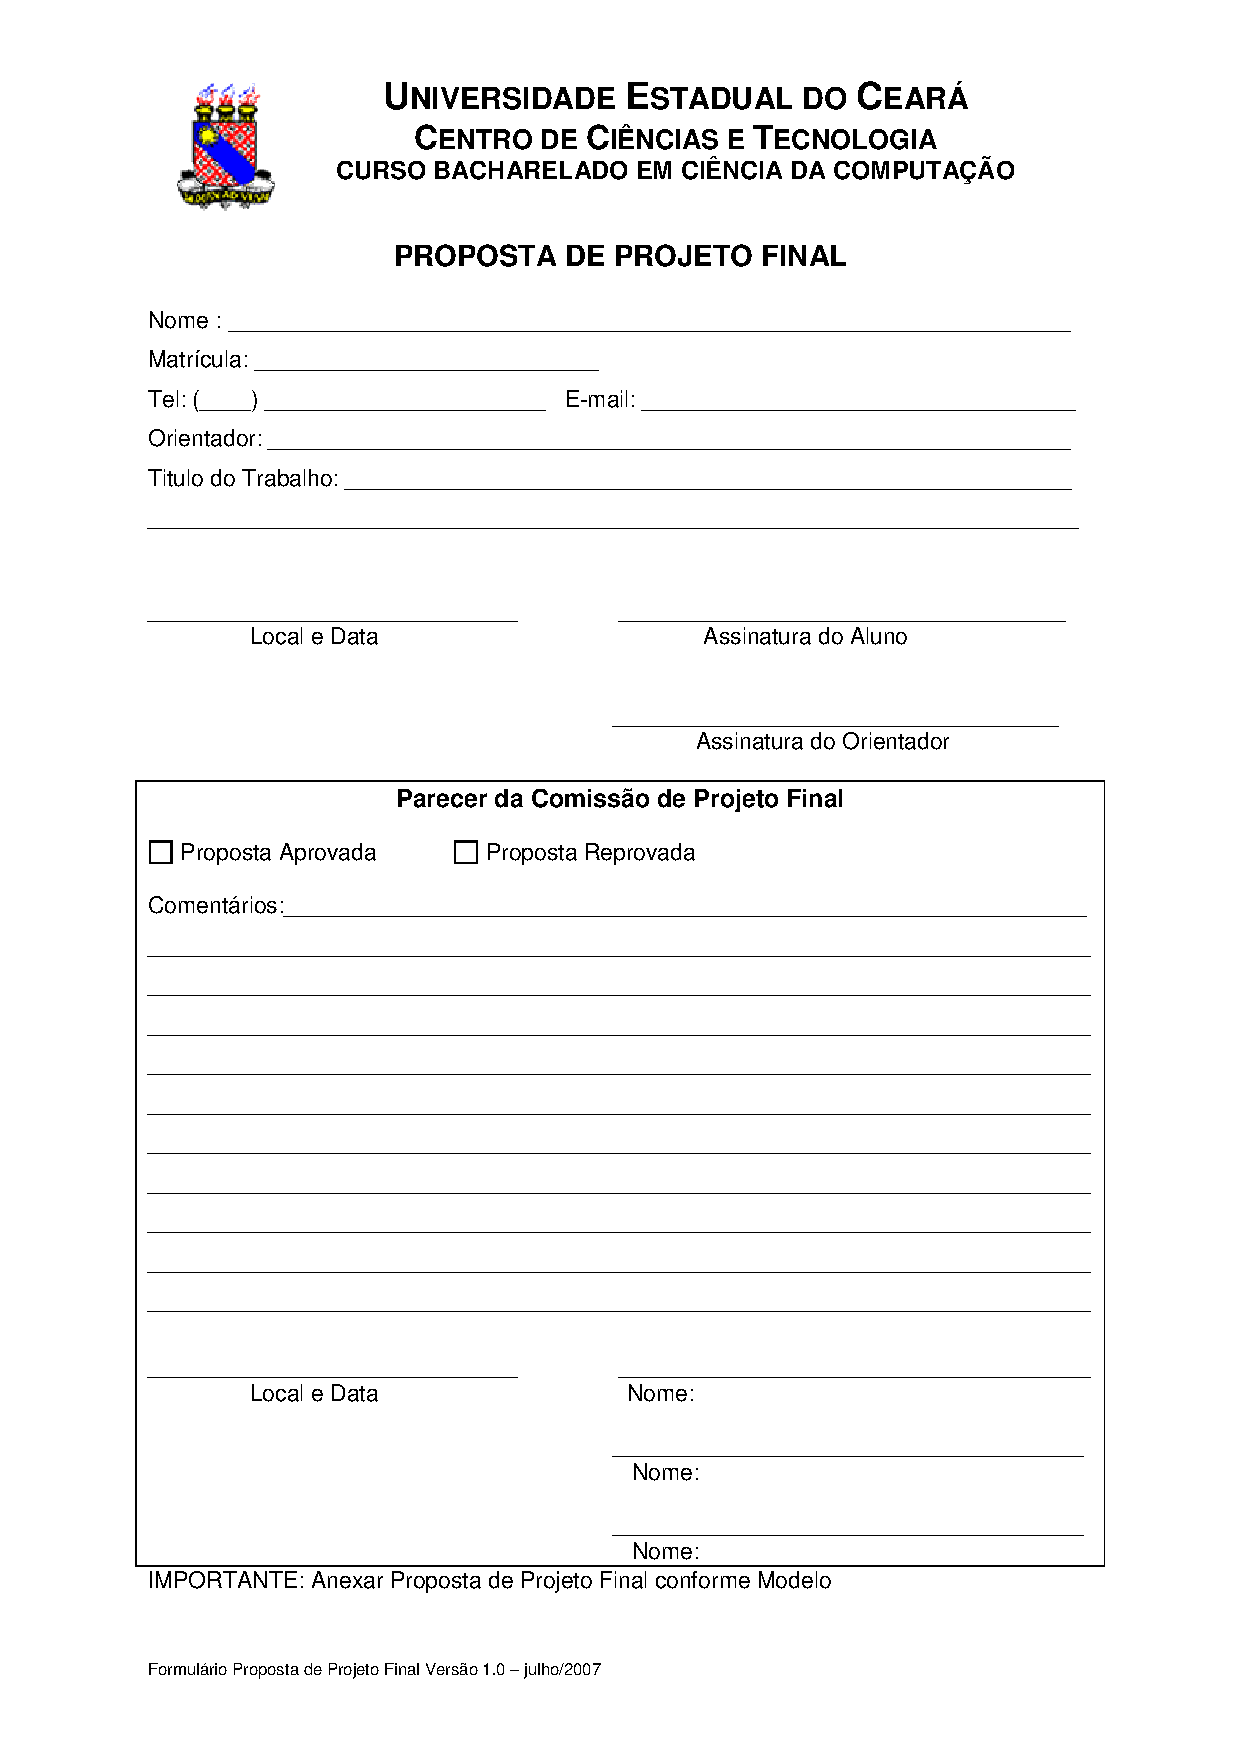
\includegraphics[scale=0.6]{requisitos/Formulario_Proposta_Projeto_Final.pdf}
\end{figure}

\clearpage
\section{Formulário de solicitação de defesa e banca}
\label{anx:defesa}
\begin{figure}[htbp]
\centering
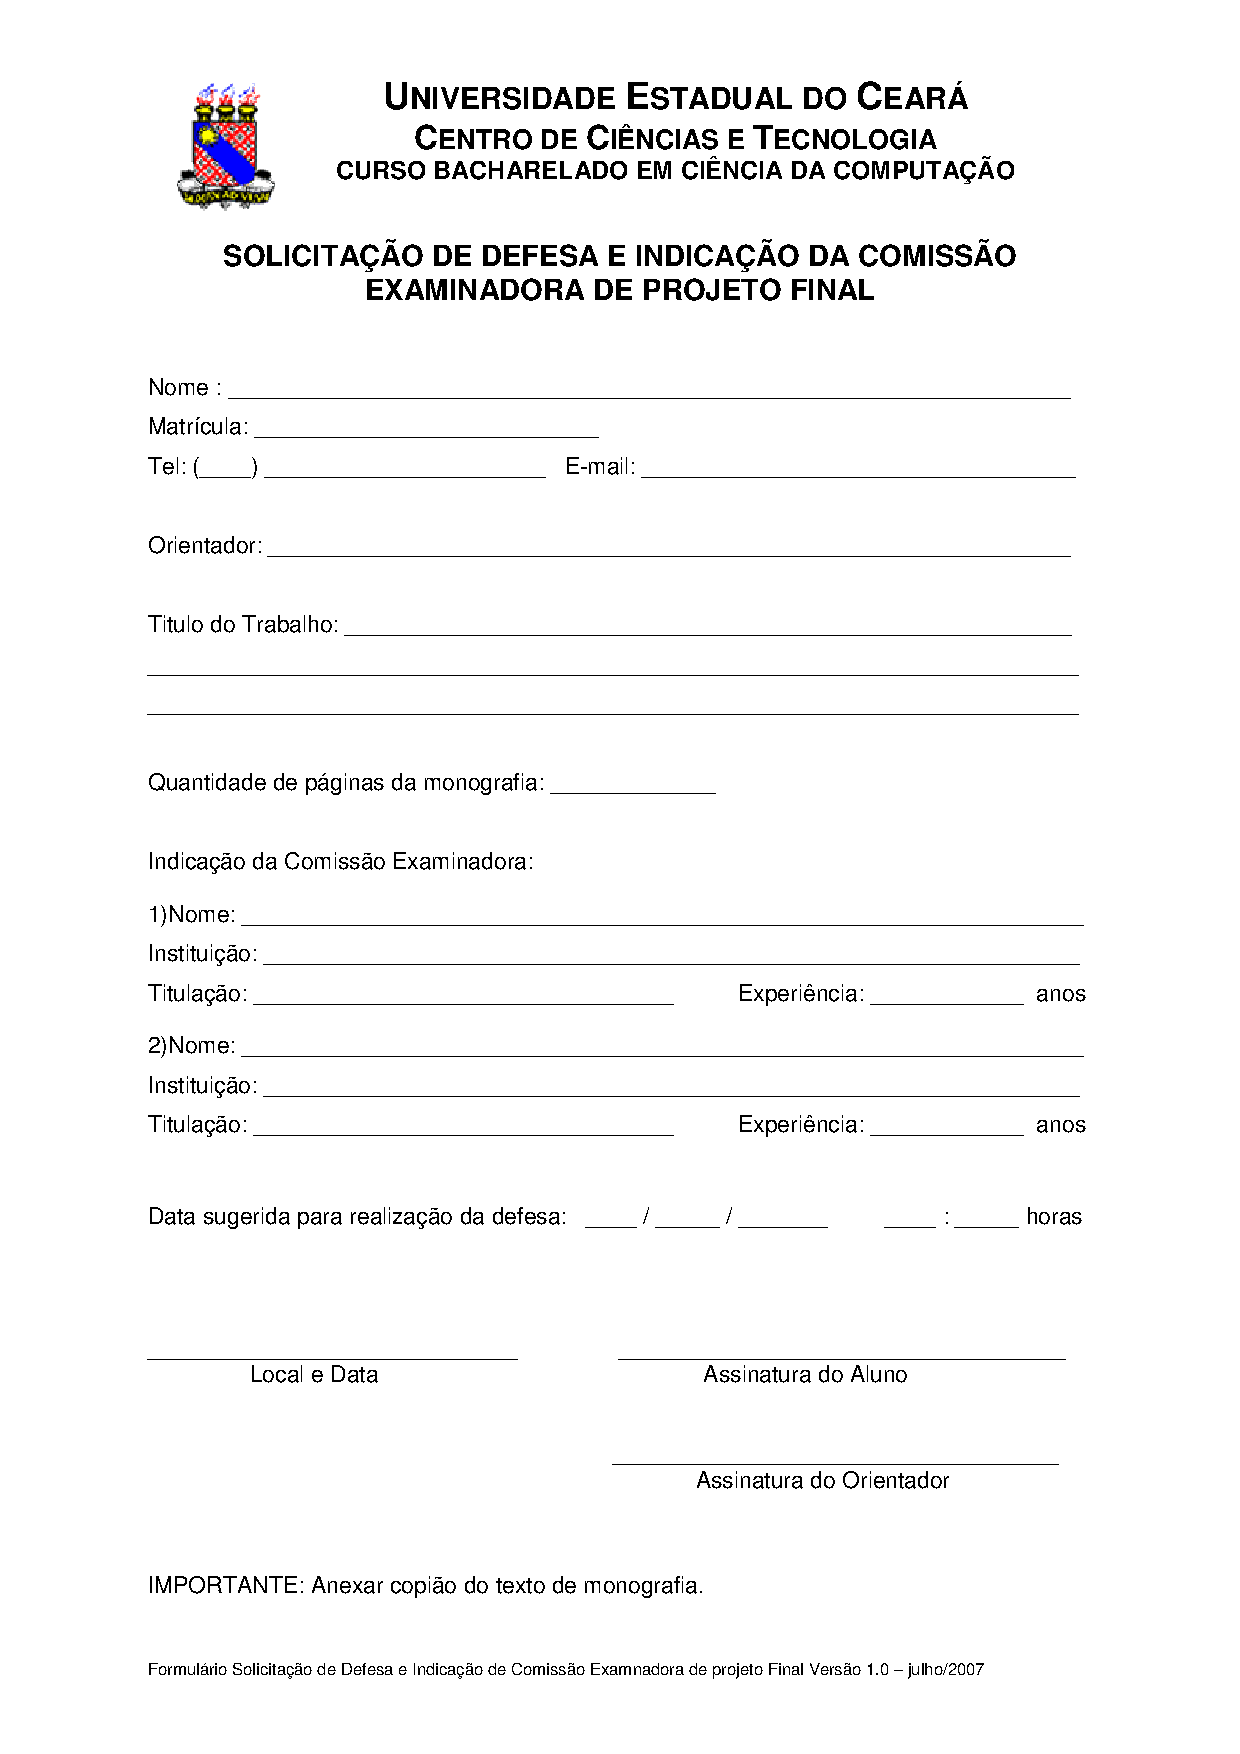
\includegraphics[scale=0.6]{requisitos/Formulario_Solicitacao_Defesa_e_Banca_v1.pdf}
\end{figure}



\chapter{Formulários}
\section{Formulário de proposta de projeto final}
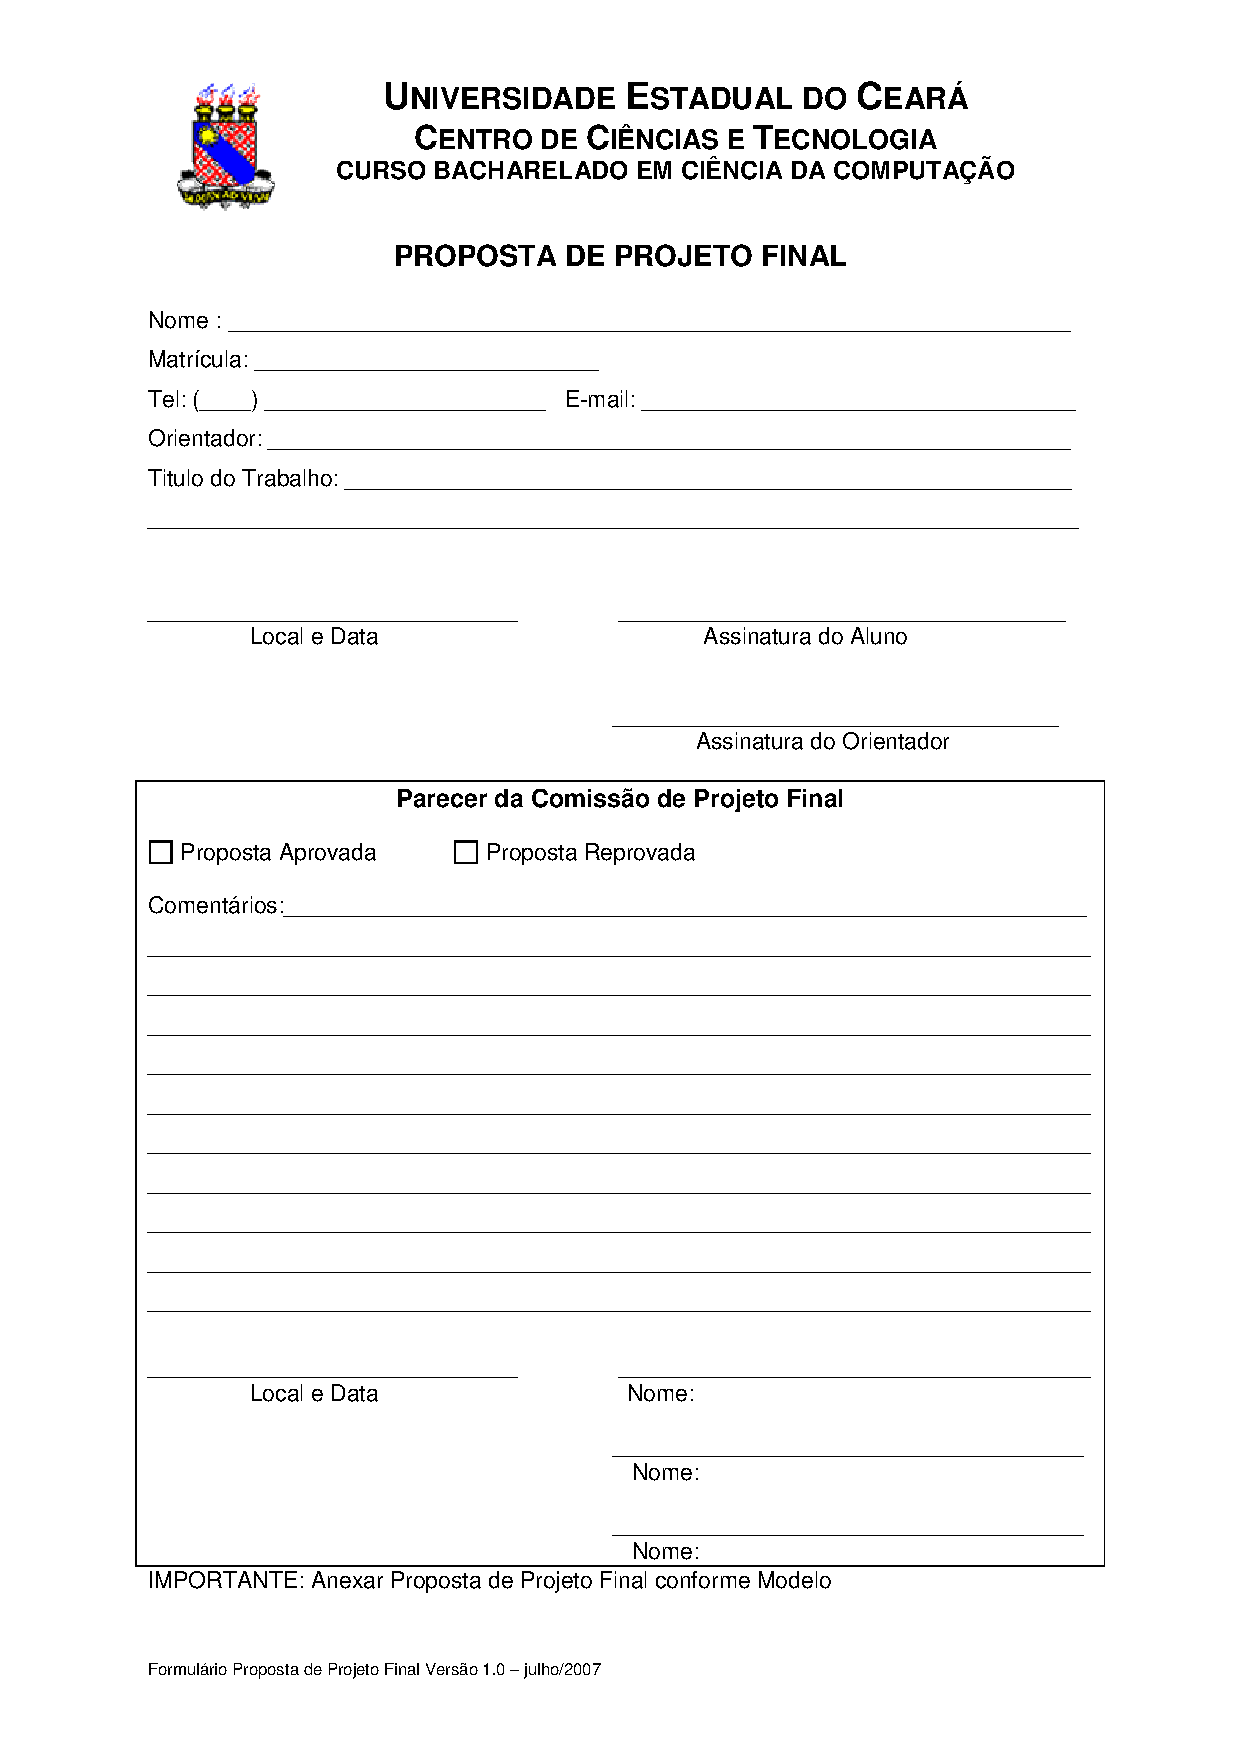
\includepdf[pages=1,noautoscale=true,scale=0.75,frame=true]{requisitos/Formulario_Proposta_Projeto_Final.pdf}

\end{document}

